% Sample file for AES paper
\documentclass{aes2e}

% Metadata Information
\jyear{2021}
\jmonth{4}



\begin{document}

% Page heads
\markboth{Gallo Robador \& Grund}{Building a synth plugin in Faust}


% Title portion
\title{SILK. Building a synth plugin in Faust }

%Author Info.
\authorgroup{
    \author{GONZALO GALLO ROBADOR},
\role{Student}
AND \author{TIM-TAREK GRUND},
\role{Student}
\email{(gonzalo.gallo@campus.tu-berlin.de)\quad\quad\quad\quad\quad\quad\quad\quad (tim.grund@tu-berlin.com)}
\affil{Technische Universität Berlin, Germany}
}

%Abstract
\abstract{%
This paper discusses the development of SILK, a synthesizer AU/VST plugin written in \textit{Faust}. It covers the \textit{Faust} code and fundamentals of the algorithms, as well as workflow routines to transfer the \textit{Faust} code into a playable AU/VST Plugin.}


\maketitle

%Head 1
\section{INTRODUCTION}
% - Rahmen (Sound Synthesis SS2020)

% - Ziel
%     - Funktionierendes Synth Plugin in DAW zum laufen zu bekommen (mit Faust)

% - Motivation

% - warum faust? Vorteile 
% (evl Website vergleichen)

% - Überblick über das Paper 
%     1. Faust Code 
%     2. Workflow zum Plugin
    

Synth plugins are used for synthesizing sounds with the help of oscillators, different waveforms, filters, modulation and other tools. They usually run within a DAW, and they are very often virtual recreations of real hardware synths. The SILK plugin is the result of our project for the course \textit{Sound Synthesis: Building Instruments in \textit{Faust}} in the summer semester of 2020 at TU Berlin. The main two goals of the project were to develop our own synthesizer in the \textit{Faust} programming language and to take it into a plugin that could be used in a DAW.

\textit{Faust} (Functional Audio Stream) is a functional programming language for sound synthesis and audio processing with a strong focus on the design of synthesizers, musical instruments, audio effects, etc., and it targets high-performance signal processing applications and audio plug-ins for a variety of platforms and standards \cite{FAUST}. Using \textit{Faust} allows us to build complex signal processing algorithms in a simple way: its compiler can ``translate" any \textit{Faust} digital signal processing (DSP) specification to a wide range of non-domain specific languages. We get a very simple syntax and great libraries that contain oscillators, effects, filters, and more ready to use. Finally, code generated in \textit{Faust} can be compiled in a wide variety of objects, such as plugins, standalone apps, or smartphone apps.

The first part of this paper talks about the \textit{Faust} code of our synthesizer. Afterward, the workflow for obtaining a plugin from there is presented.

\section{Faust Project}
In this section we explain the code and algorithms of the \textit{Faust} project for SILK.

\subsection{Features Overview}
SILK has three wave generators, four waveforms (sine, triangle, square and sawtooth), a subtractive filter, AM modulation, an ADSR envelope, reverb, and supports up to 32 simultaneous voices (see Figure \ref{fig:silk_gui_qt}).

\begin{figure}[h]
\centering
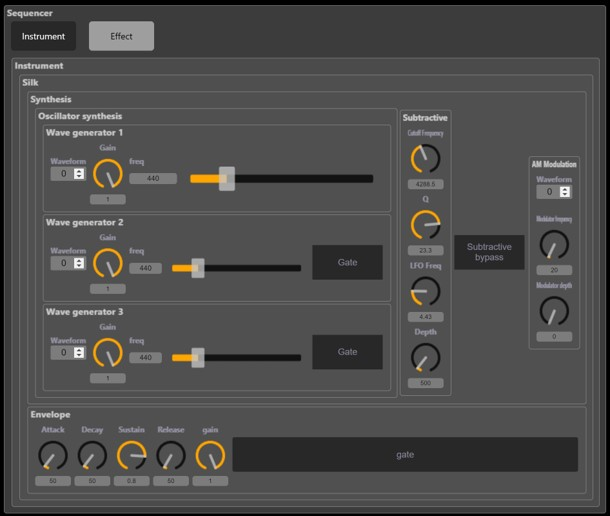
\includegraphics[width=0.35\textwidth]{Figures/silk-gui-qt.jpg}
\caption{Qt interface of the SILK synthesizer in the \textit{Faust IDE}}
\label{fig:silk_gui_qt}
\end{figure}

\subsection{Process Line}
Before we dive into the individual parts that are involved in the signal processing of our synthesizer, let's take a look at the bigger picture. The most fundamental part of any \textit{Faust} program is the \textit{process} line. In this part of the code, we pass the desired inputs and outputs to the target. This is a dynamic system, meaning that we can just type in any number and arrangement of inputs and outputs at the right side of the equal sign, and it will adjust to it providing the program with inputs and outputs as needed \cite{FDOC}.

The diagram in Figure \ref{fig:process} shows the last stage of the process line. The block named \textit{synthTypes} contains the output signal of the sound synthesis process in our synthesizer. The envelope is applied to our signal using the multiplication box and after that, the line splits in two. These two lines will be used as an input by the \textit{effect} element (see Section \ref{subsec:reverb} for more about this).

\begin{figure}[h]
\centering
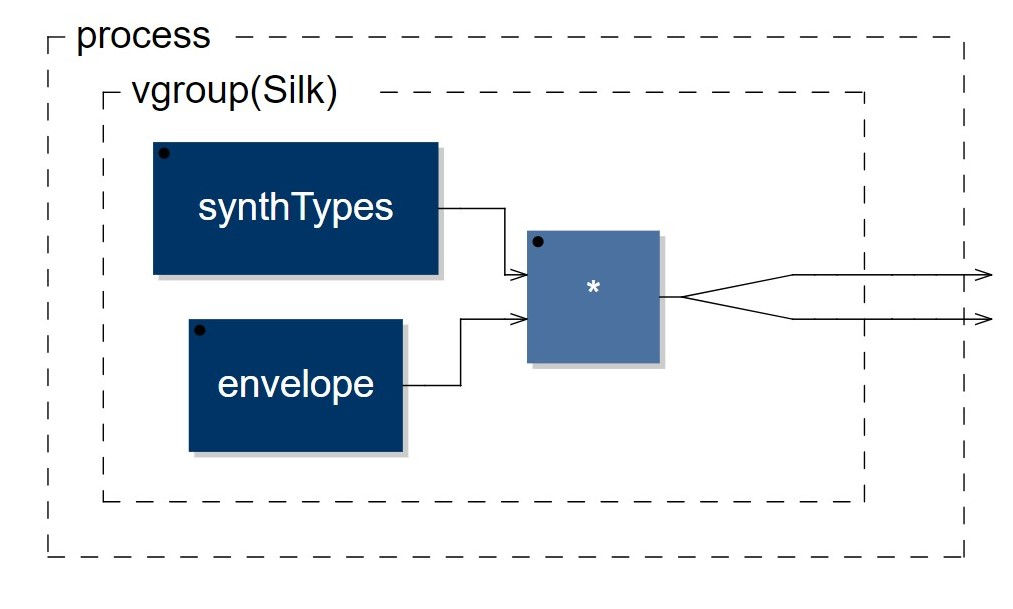
\includegraphics[width=0.3\textwidth]{Figures/process.jpg}
\caption{Diagram of the process line: Sound synthesis output and envelope}
\label{fig:process}
\end{figure}

If we take a look inside the \textit{synthTypes} block, we will see the diagram shown in Figure \ref{fig:process1}. Here, the oscillator synthesis signal (\textit{oscSynth}) is multiplied by the AM (\textit{amMod}) and the subtractive filter (\textit{vcf}), with the particularity that the latter can be bypassed.

\begin{figure}[h]
\centering
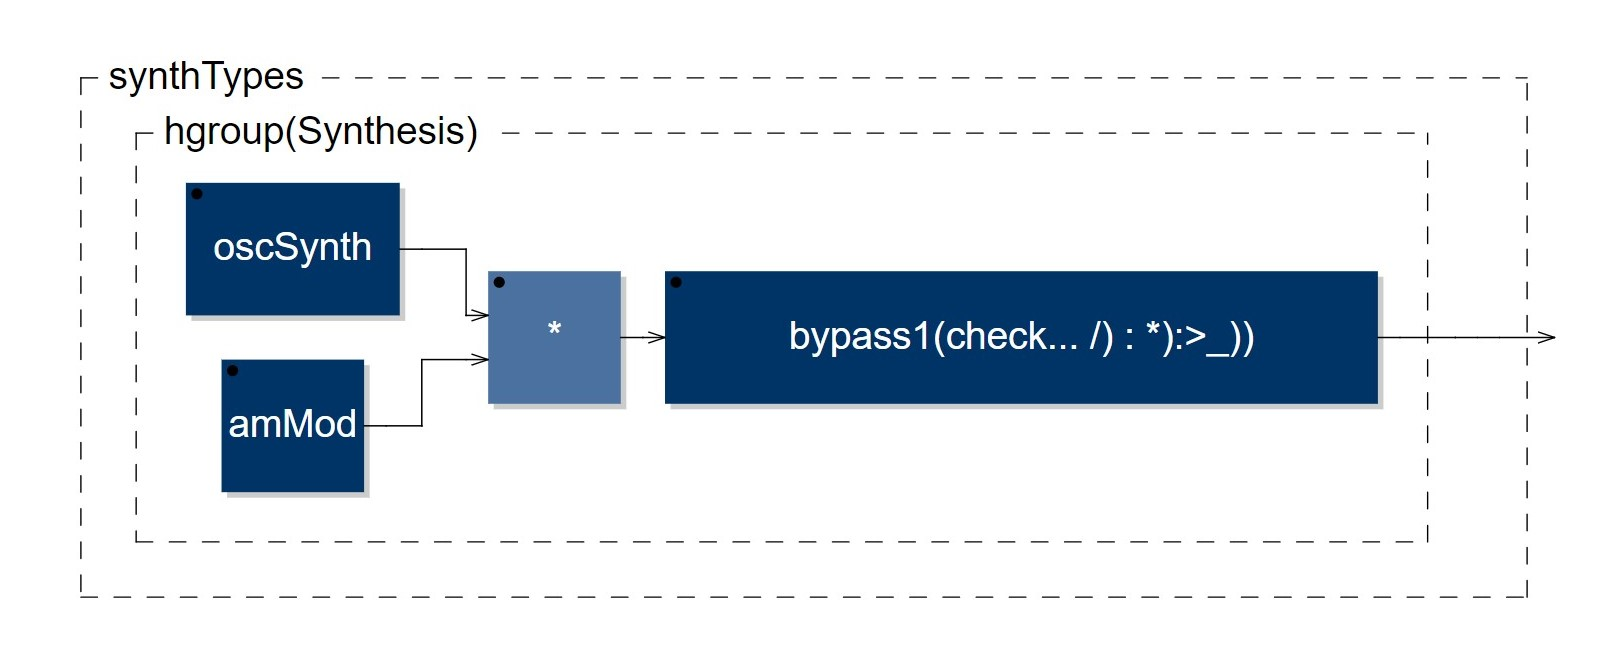
\includegraphics[width=0.45\textwidth]{Figures/process1.jpg}
\caption{Diagram of the process line: Oscillator Synthesis, AM and subtractive filter}
\label{fig:process1}
\end{figure}

\subsection{Oscillator Synthesis}

The basic \textit{Faust} code that is used for generating waves in SILK is presented in Figure \ref{fig:osc_synth_1}. In lines 13 to 16, we define the four different waveforms that will be available for synthesizing sound: sine, triangle, sawtooth and square. For the sine and triangle waves we added overtones in order to obtain a richer tone.

\begin{figure}[h]
\centering
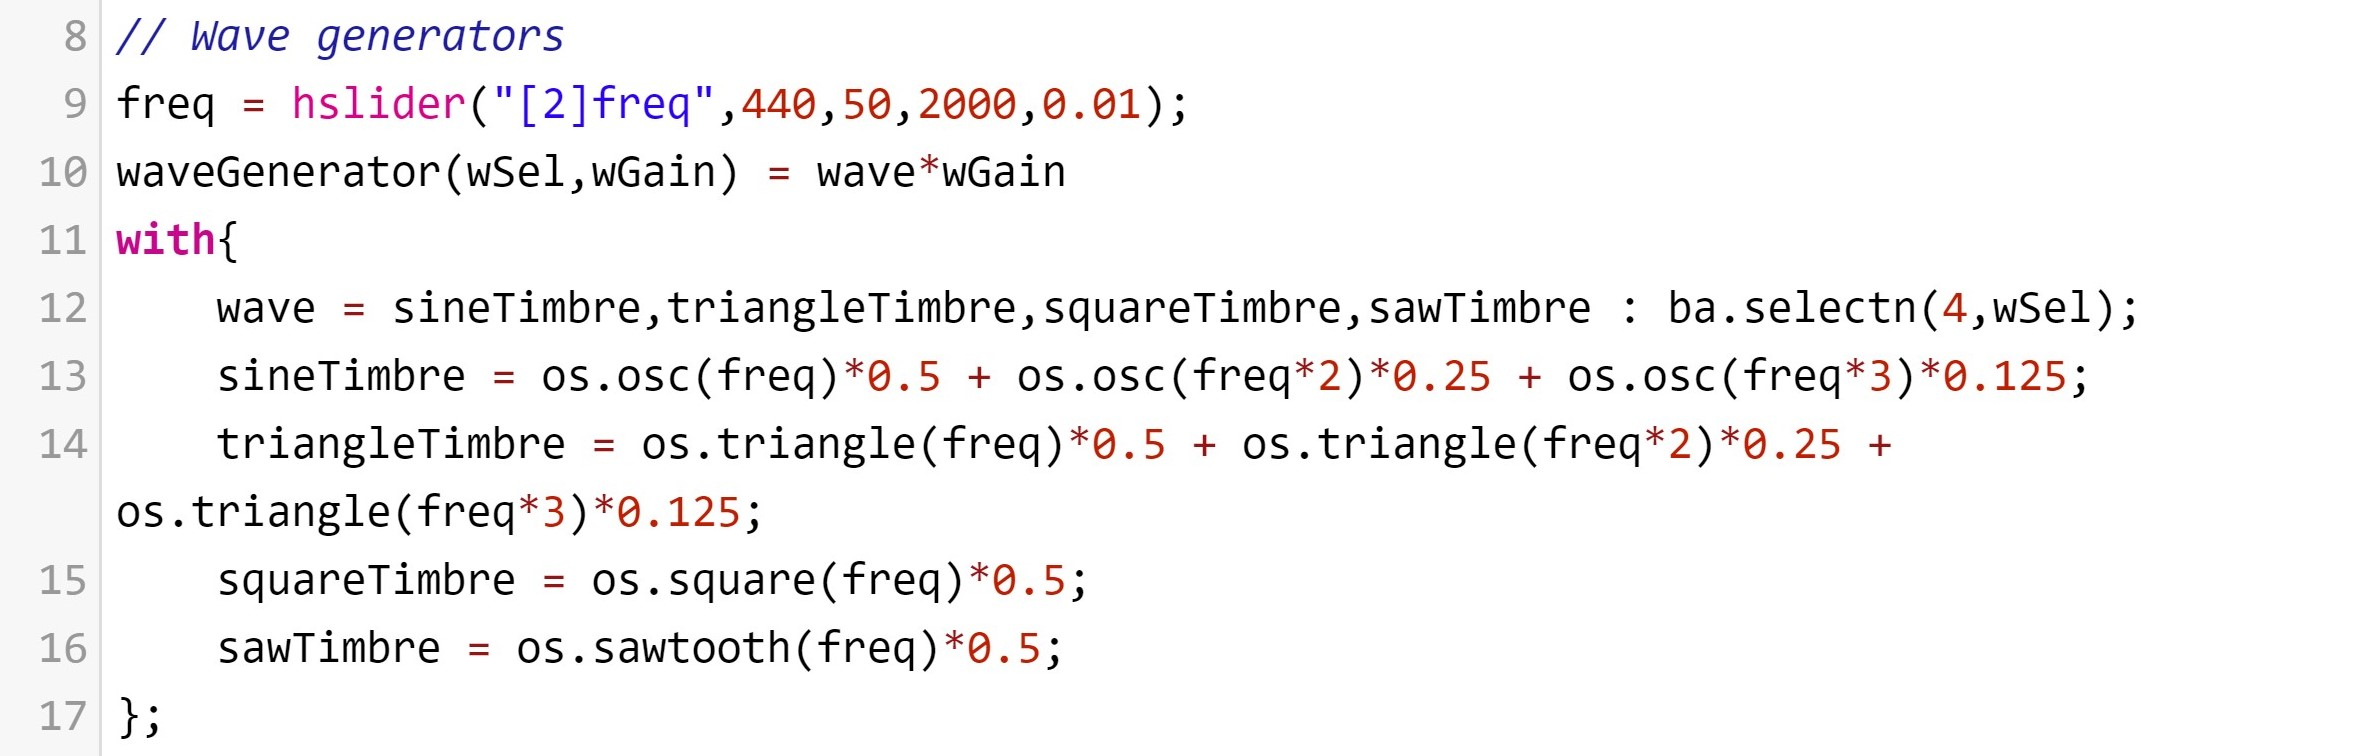
\includegraphics[width=0.5\textwidth]{Figures/osc_synth_1.jpg}
\caption{Defining the waveforms: Generic \textit{Faust} function \textit{waveGenerator}}
\label{fig:osc_synth_1}
\end{figure}

Subsequently, three wave generators are created using this generic \textit{waveGenerator} function (see Figure \ref{fig:wavegens}). Having multiple wave generators to use simultaneously allows users of SILK to further shape their own tone.

\begin{figure}[h]
\centering
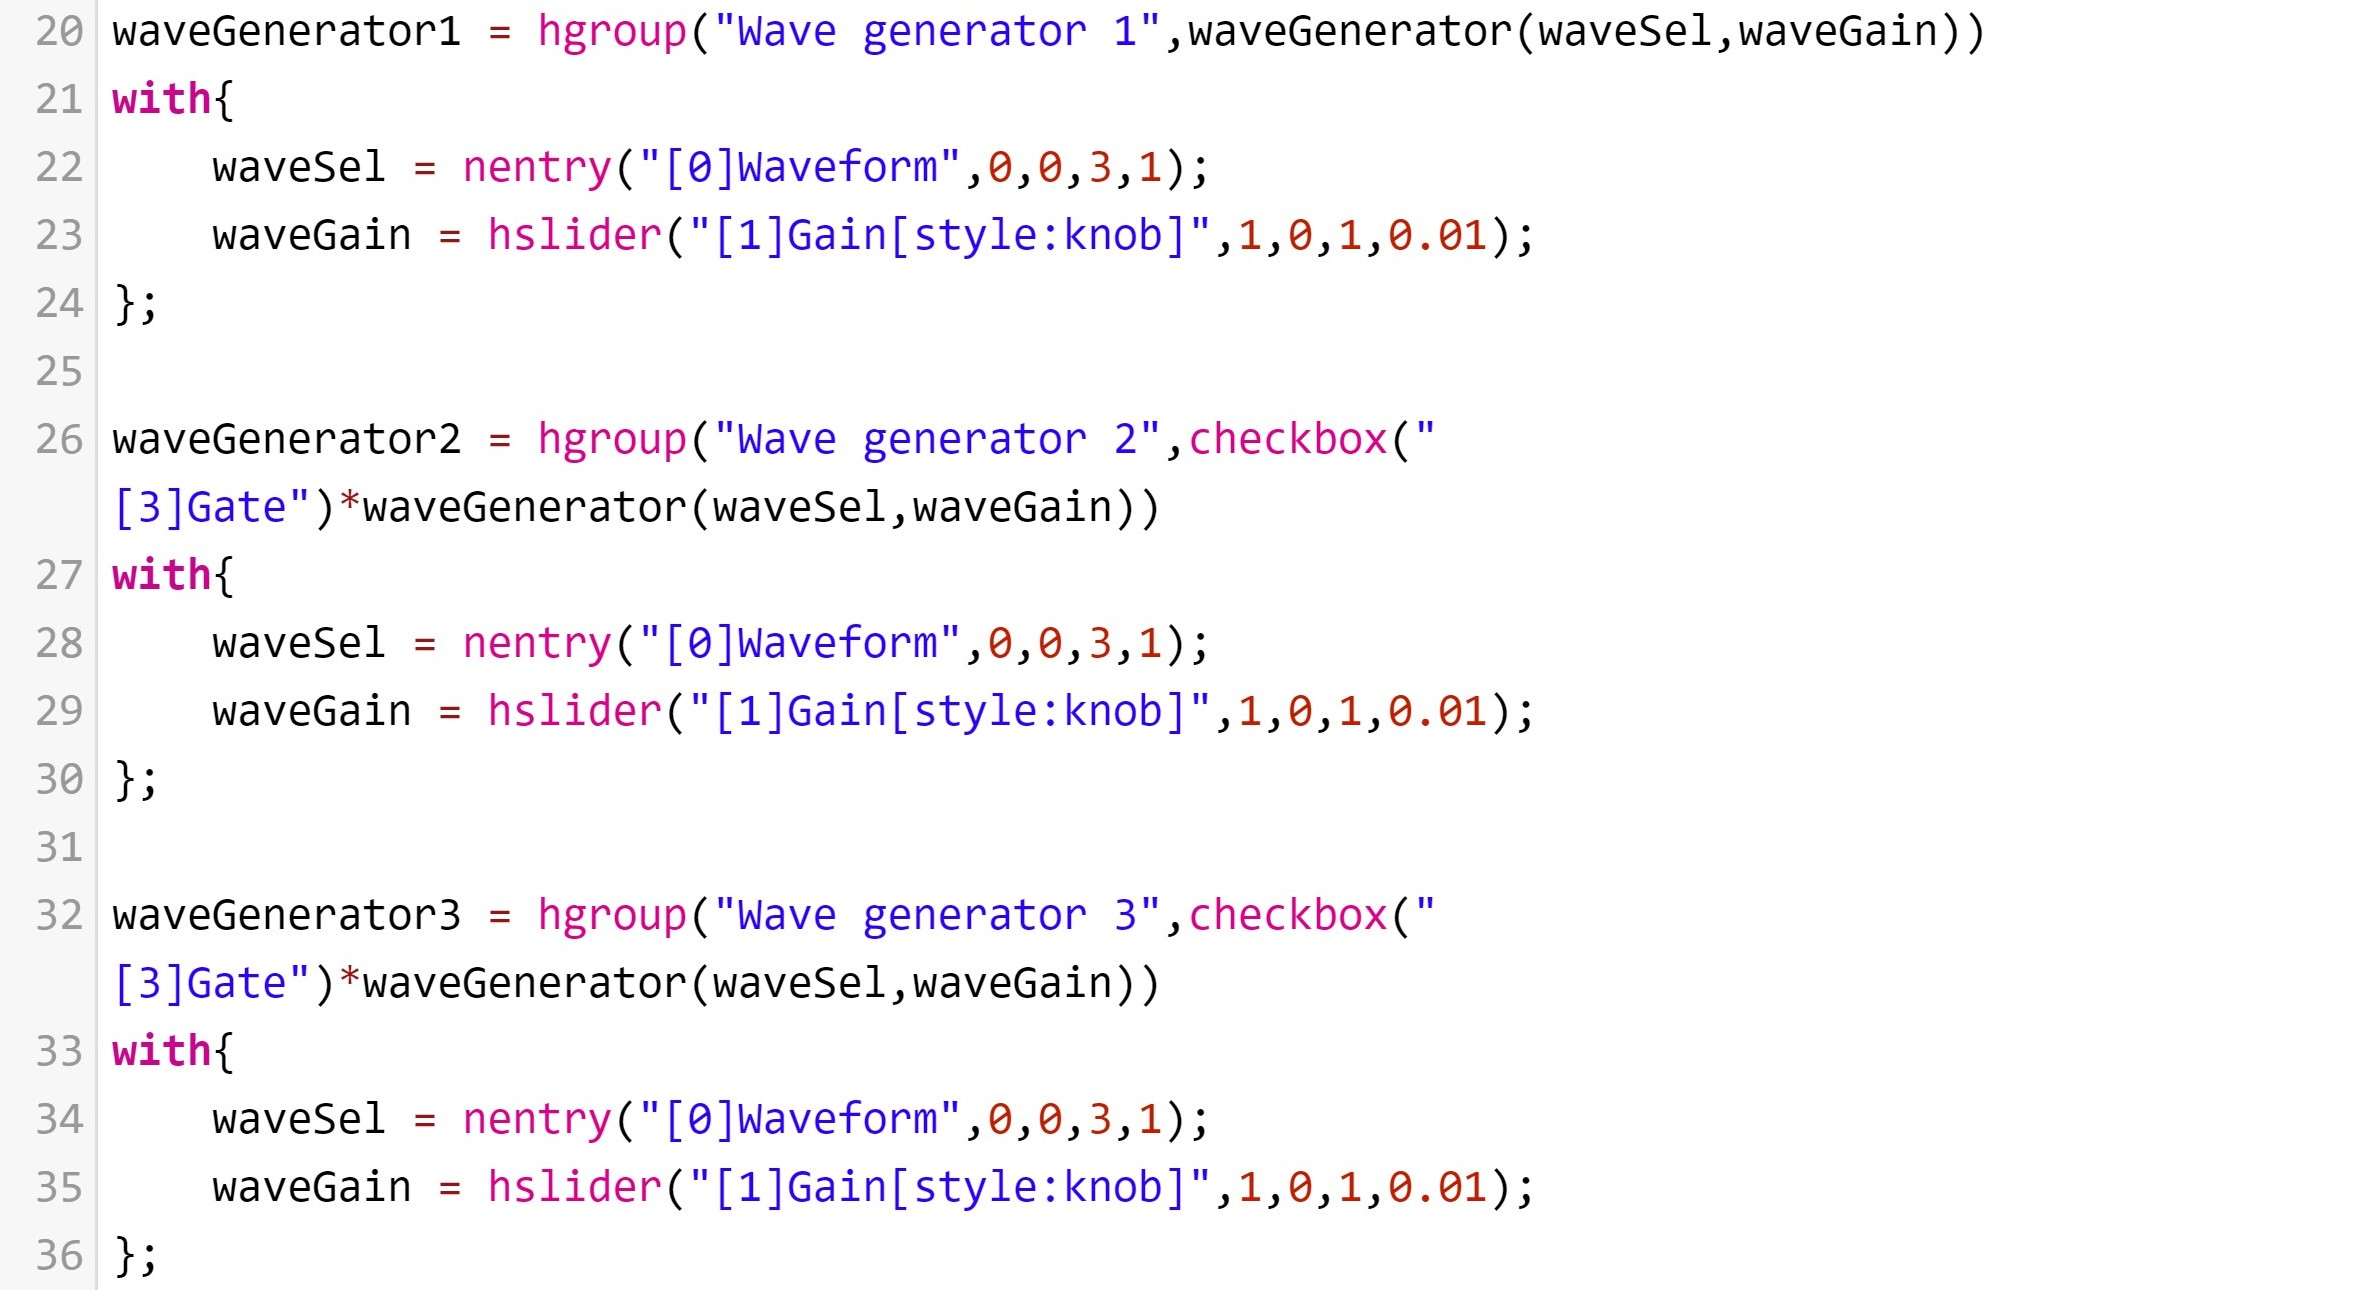
\includegraphics[width=0.5\textwidth]{Figures/wavegens.jpg}
\caption{Creating three wave generators using the generic \textit{waveGenerator} function}
\label{fig:wavegens}
\end{figure}


\subsection{AM Modulation}
AM (Amplitude Modulation) consists in modulating the amplitude of a given wave with another wave that is called \textit{modulator}. The \textit{Faust} code for the implementation of the AM in SILK is presented in Figure \ref{fig:am_mod}. 

\begin{figure}[h]
\centering
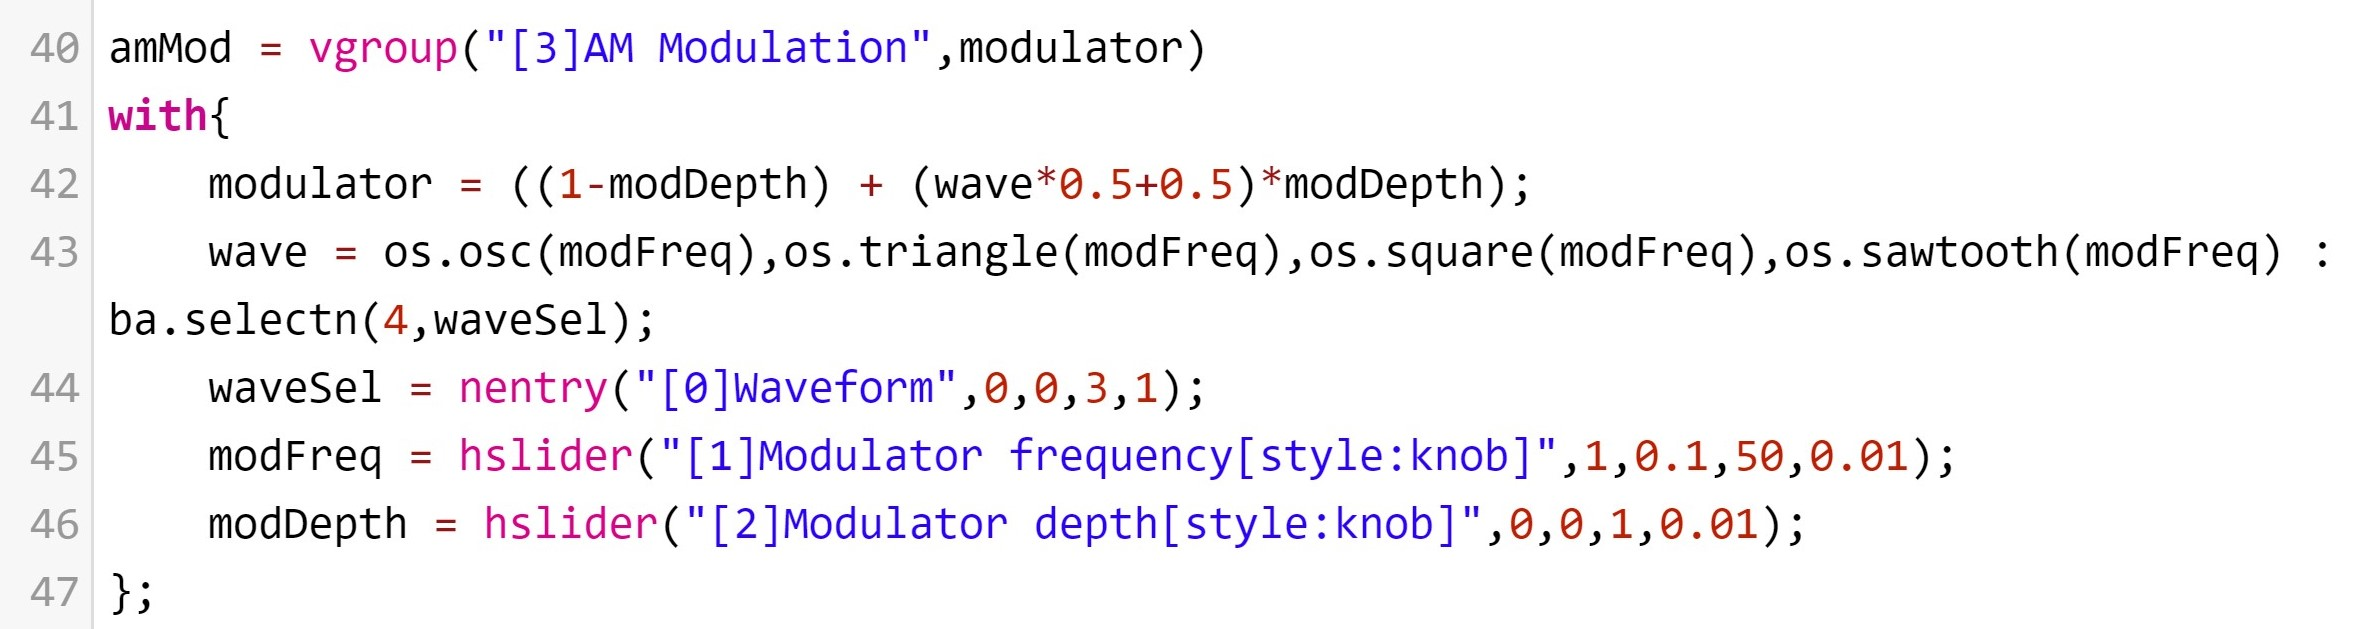
\includegraphics[width=0.5\textwidth]{Figures/am_mod.jpg}
\caption{AM Modulation}
\label{fig:am_mod}
\end{figure}

To which extent the modulation is done, is specified by the \textit{modulation depth} parameter. We are also able to choose which waveform we want to use for modulating, and at which frequency.

\subsection{Subtractive Filter}
Subtractive synthesis is the process of taking an initial, harmonic-rich tone, and subtracting parts of it using filters and other tools in order to create a musical timbre\cite{SUBT}. Our synth has a virtual \textit{vcf} (Voltage Controlled Filter) that has four parameters: \textit{cf} (cut-off frequency), \textit{q}, \textit{lfoFreq} and \textit{lfoDepth} (see Figure \ref{fig:sub_fil}). We take advantage here of \textit{fi.reson.lp}, a simple resonant lowpass filter based on tf2s (virtual analog) of the \textit{Faust} libraries.

\begin{figure}[h]
\centering
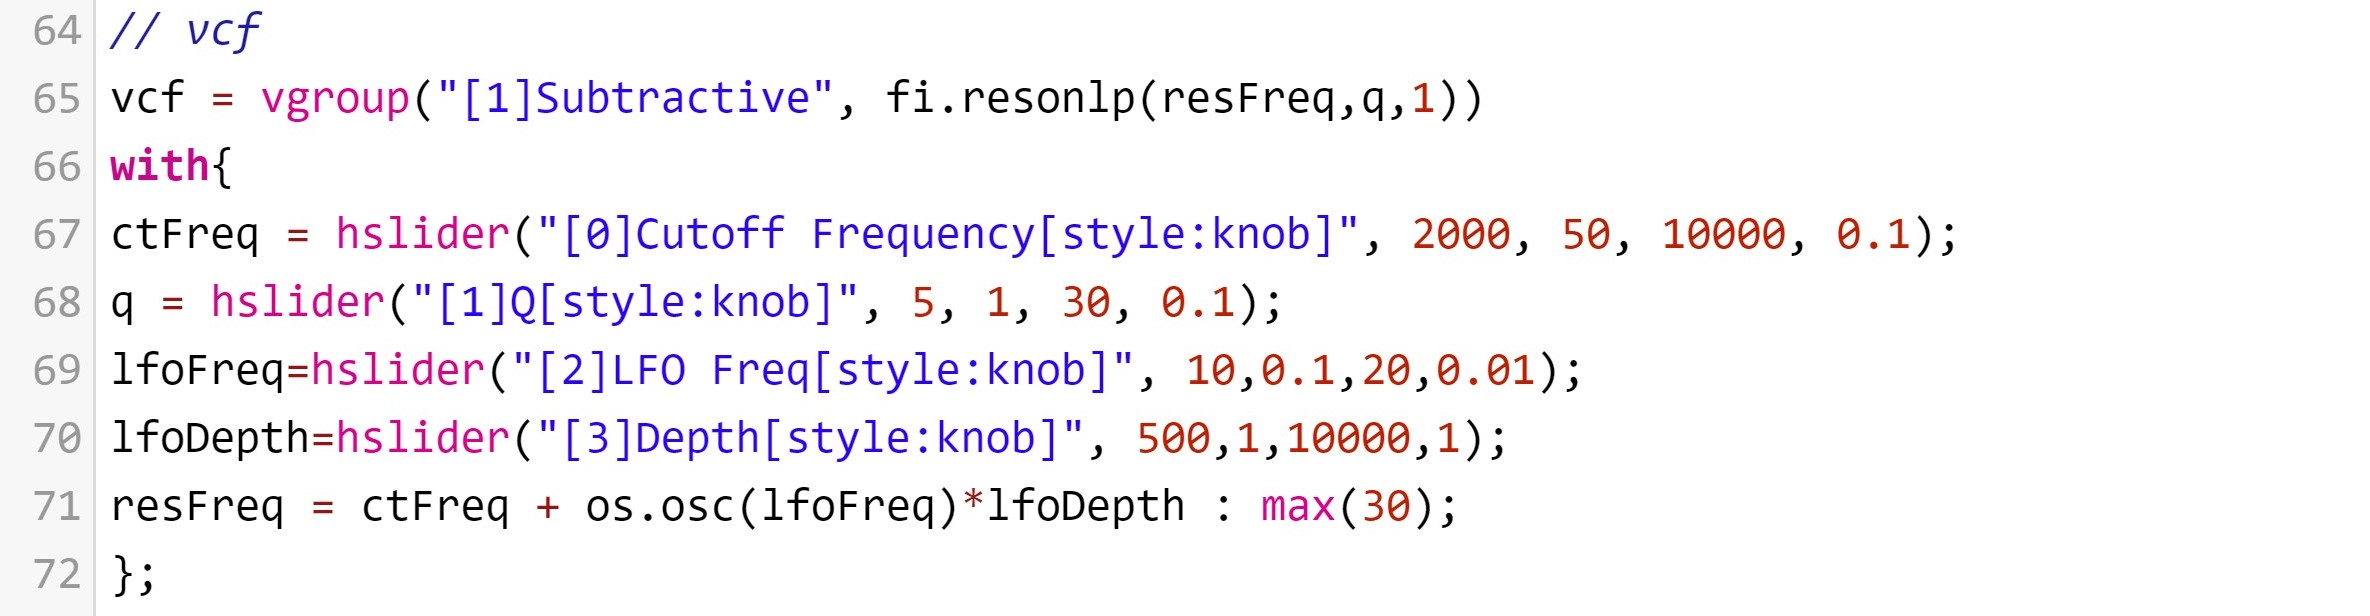
\includegraphics[width=0.5\textwidth]{Figures/sub_fil.jpg}
\caption{Subtractive Filter}
\label{fig:sub_fil}
\end{figure}

\subsection{Envelope}
The SILK integrates an ADSR envelope at the final stage of the process line (see Figure \ref{fig:process}). ADSR envelopes (\textit{Attack, Decay, Sustain} and \textit{Release}) are the usual way to implement gain envelopes in synthesizers, and they basically set a time for each of the \textit{attack}, \textit{decay} and \textit{release} parameters and a percentage for the \textit{sustain} one.

An ADSR envelope can be easily implemented in \textit{Faust}. We just have to use the \textit{adsr} object of the envelope library in \textit{Faust} (see Figure \ref{fig:envelope}).

\begin{figure}[h]
\centering
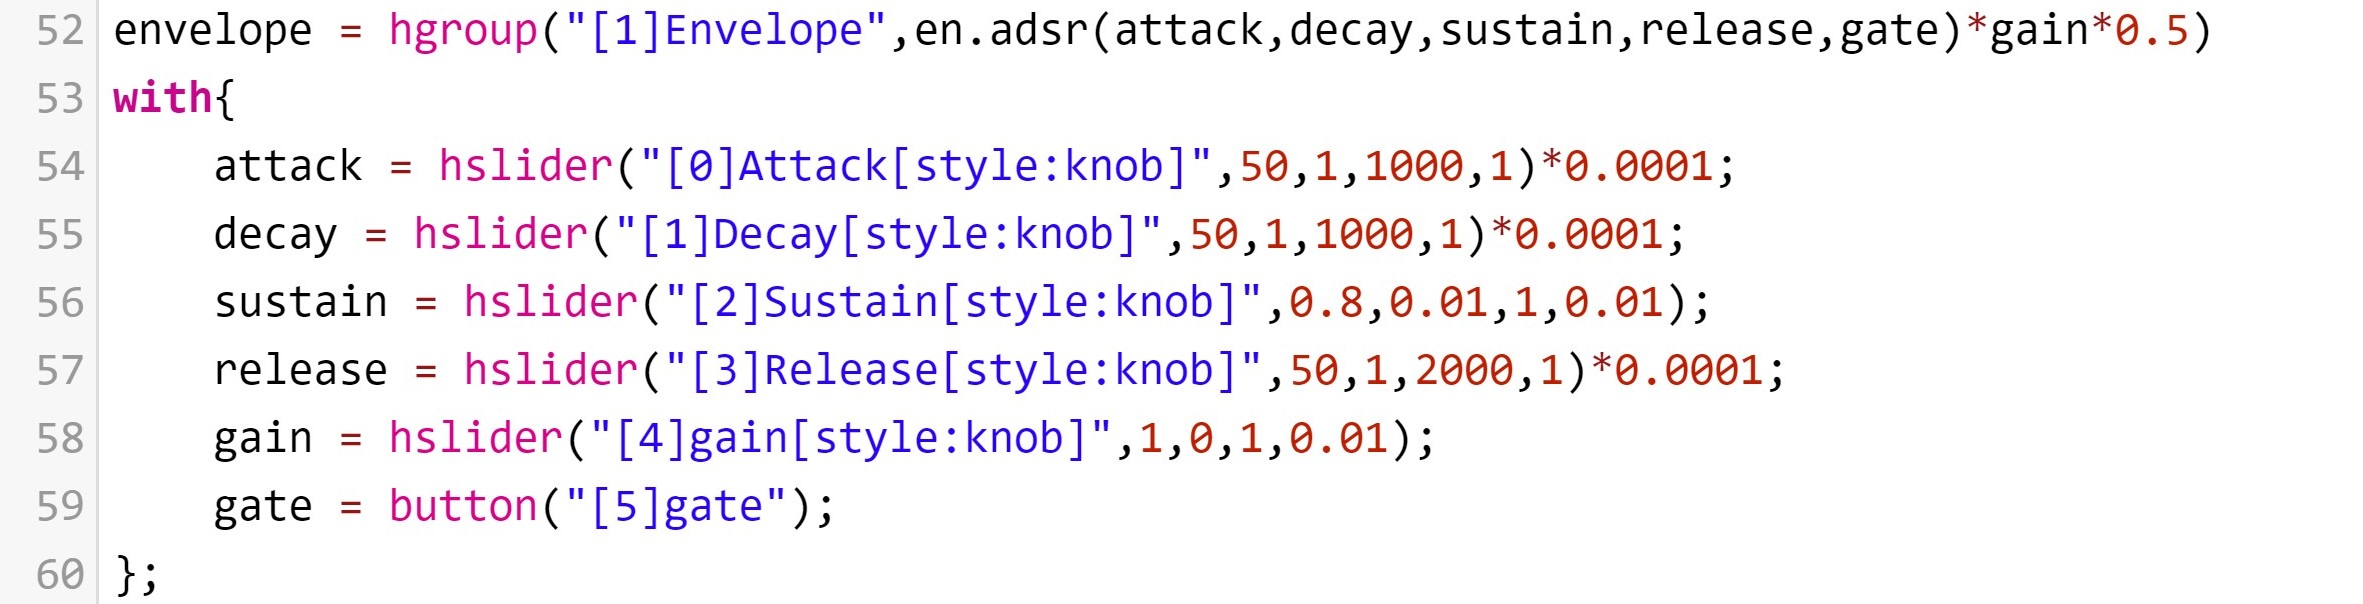
\includegraphics[width=0.5\textwidth]{Figures/envelope.jpg}
\caption{ADSR envelope in \textit{Faust}}
\label{fig:envelope}
\end{figure}

\subsection{Polyphony}
If we take a closer look at the code of the envelope, we see that we have multiplied the gain of our envelope by 0.5 (see figure \ref{fig:envelope}). This is because synthesizers make use of polyphony, that is, several notes played at the same time. If we do not reduce the overall gain of our process line, the gain of the different notes will add up without being scaled, which can end up causing clicking.

In order to enable our program to receive MIDI input, we have to set the \textit{Poly Voices} field in the configuration of the \textit{Faust} compilation to the desired number of simultaneous voices. By default this is set to \textit{Mono}, which doesn't take any MIDI input. For our synthesizer, we set it to 32 voices.

\subsection{Reverb}
\label{subsec:reverb}
So we already have a polyphonic synth and we want to add a reverb. We might be tempted to put a reverb element at the end of our process line, but that would be wrong. It would be very inefficient, because it would apply the effect to each single note. Instead, by defining an \textit{effect} element anywhere in the code, a global audio effect will be applied to all the polyphonic voices at once. Also notice that the number of outputs of our process line has to be the same as the inputs to the effect line. We used the \textit{zita\_light} reverb (see Figure \ref{subsec:reverb}), that has a stereo input, and thus we have to provide two outputs at the end of our process line (See figure \ref{fig:process}).

\begin{figure}[h]
\centering

\includegraphics[width=0.5\textwidth]{Figures/audio_effect.jpg}
\caption{Audio effect in \textit{Faust}}
\label{fig:audio_effect}
\end{figure}



\section{IMPLEMENTATION}
There are several approaches to generating a plug-in instrument using FAUST. Since our goal was to have the synth usable for audio production inside a Digital Audio Workstation (DAW) and we had access to Logic Pro X, which only supports the Audio Unit format (AU) natively, we decided to aim for this format. 
Because there exists the faust2au script, which should provide a great FAUST plug-in in the desired format, our first attempt included trying to get this approach to work. However, at the time of the project (Summer 2020), we were not successful in this approach, which led us to trying the alternatives we will introduce in this paper.
The different approaches yield different results and come with individual advantages and drawbacks which we will examine, too.

\subsection{faust2vst}
The first workaround we employed is a fairly simple approach to the problem of Logic Pro X not being able to utilize other formats besides AU: We build a plug-in in the vst format using the faust2vst script and run it using a wrapper plug-in.
We developed the code in the \textit{Faust IDE} online editor, which held the advantage of not needing to install Steinberg's vst development kit.
Using the \textit{Faust IDE's} option to export and compile to a specific platform binary code, we chose \textit{osx} as the platform and \textit{vst} or \textit{vsti} as the architecture.
Unlike the aformentioned faust2au script, the vst option built without any problems.
After exporting using the \textit{\textit{Faust} IDE}, we can now download the export. The download contains the vst(i) file as well as a makefile and the FAUST code.
We now place the vst file in the folder, that is at the end of the path, where our DAW scans for vst plug-ins. 
For Mac users it should be Library $>$ Audio $>$ Plug-Ins $>$ VST.
If your DAW is already able to run vst plug-ins, you are now set and ready to go. However we now still had to translate our plug-in to the AU format.
To achieve this we had to make use of a plug-in, that is able to run other plug-ins, especially vst plug-ins. For this purpose we used DDMF's Metaplugin \cite{DDMF2021}. 
In the following section we will discuss the the steps taken using Metaplugin, however we believe that using other wrapper plug-ins will result in a similar workflow.

Firstly we have to open Metaplugin inside our DAW.
Since we are using Logic, we select the instrument slot inside the channel-strip. Here, we select AU-Instruments $>$ DDMF $>$ MetaPluginSynth. 
If you are building an effect plug-in, make sure to open Metaplugin from the Audi FX space, choosing Audio Units $>$ DDMF $>$ Metaplugin.
If the plug-in is not available in the menu, you may need to rescan your plug-in by choosing Logic Pro $>$ Preferences $>$ Plug-In Manager, or MainStage $>$ Preferences $>$ Plug-In Manager (if you are using Logic Pro X as well).

Secondly, having opened the MetaPluginSynth, we check whether our vst is available. If it is not, we need to scan inside the plug-in. To do so, we select Options > Scan for new or updated VST plug-ins. You might need to select which folder to scan. Choose the one in which you have placed your vst file.
If you are using a Mac, you might encounter the problem of macOS not being able to verify whether your vst file contains malware, which results in your vst file not being opened inside the Metaplugin. You can choose to open it nevertheless from your safety settings. Once your mac has tried opening it from the safety settings, you can scan again and continue.
3. Now our plug-in is visible inside the MetaPluginSynth, from where you can open it. Make sure to connect your plug-in with the required in- and outputs inside the MetaPluginSynth.
Your plug-in should be ready to use now.

At the time of this project (Summer 2020) we encountered a few problems regarding this workflow: The most noticeable one may be that, contrary to the GUIs of of other targets, all elements of the GUI of the final vst are sliders that are placed below each other, making layout of and operating the synth significantly counterintuitive. Furthermore, the slider values are all placed between zero and one, which makes precise settings fairly difficult.

Another drawback of this workaround is the missing midi support: In order to actually play our synth, one has to select the frequency and other parameters using the sliders beforehand and move the main gate slider above the .5 threshold. This is due to the GUI element of a switch being turned into a slider element.
However, this approach also has a lot of advantages: The time it takes to move from FAUST code to a usable plug-in is considerably fast, making it useful for prototyping and testing FAUST coded plug-ins. There is also, apart from FAUST knowledge, no further coding knowledge required, making it easy for beginners to built a plug-in by themselves. There is also no need for additional installations and further programming.
We believe that despite the shortcomings regarding the missing MIDI functionality the workflow still holds value especially for audio effects development. However, the challenging layout and operating might prove useful or inspiring for the creation of drone sounds.

\subsection{faust2juce}
This approach consists of three steps:
\begin{enumerate}
    \item Getting a basic Juce plug-in running in Logic Pro X
    \item Exporting the FAUST code as faust2juce
    \item Adding the faust2juce code to the juce project.
\end{enumerate}
As with the preceeding workflow of faust2vst, this approach works on a Mac with Logic Pro X. In addition Xcode and JUCE are needed to follow through with this example. Another IDE might work as well, you might however need to take extra steps.

Firstly, we install JUCE \cite{JUCE2021} and open up the Projucer. There we select New Project $>$ Plug-In $>$ Basic, choose a name and click 'Create Project'.
Now we set all module paths to global and select Xcode as our selected exporter. 
Inside of the settings under Plugin Characteristics we select 'Plugin is a Synth', 'Plugin MIDI Input', and 'Plugin MIDI Output'. We now add a company name and click on the button to open the project inside our preferred IDE.
When using Logic Pro X, the company name decides where a plug-in can be found inside of Audio FX $>$ Audio Units in the Channel Strip.
Now in Xcode, we change the scheme to 'AU' using the dropdown menu in the upper left corner. Inside the same menu, we select 'Edit Scheme'. We now select Logic Pro X (our preferred DAW) as our executable. This allows us to automatically open up the plug-in inside of our DAW once Xcode finishes building. We now deselect 'debug executable'.
Finally, we can press 'Build' and open up Logic Pro X. Occasionally, a plug-in cannot be found under a specified company name. In this case, deleting the cache file under Library $>$ Caches $>$ AudioUnitCache and restarting the Mac might work. Upon reopening Logic Pro X, the program should automatically scan the plug-in.
We should now be able to open the plug-in. It should contain a blank space and the text "Hello World!".
Since we are building our workflow around using JUCE, it takes more time learning and the start-to-end process is also delayed. However, JUCEs varied possibilities ultimately allow for the user to customize their GUI with far more precision than other workflows.

\section{CONCLUSION}

%Ziel erreicht
Ultimately, we have managed to achieve our goal of building a functional synth plugin and running it in our DAW. However, our approaches contained some drawbacks: The playability of the synth is limited, due to missing compatibility with MIDI inputs. Also, our processes of compiling the FAUST code to a certain target and taking it from there to a plugin format proved to be a little challenging for coding beginners, although one could argue, that starting coding in general can be considered tedious, independent of plattforms. We hope that this paper adds to the body of knowledge concerning FAUST and aids the simplification of getting started. 
%Mit Nachteilen:
%    - Spielbarkeit der Synths begrenzt
%    - Kompilieren in bestimmtes Format nicht ganz anfängerfreundlich
Nevertheless, using FAUST provided quite a few opportunities for programming and prototyping use: the language itself demonstrates ease of use due to its intelligibility. Adding to the diverse capabilities of FAUST, the supporting libraries greatly increased the scope of application and reduced programming efforts. Accelerating the workflow especially for beginners, even considering the obstacle of challenging workflows is also a major benefit of FAUST.
Considering the missing MIDI support of our workflow we can take a look at the existing body of knowledge present. Apparently, Weiß and Körwer \cite{Weiss2020} managed to find a workflow providing MIDI support for FAUST based plugins.
%- Vorteile:
%    - Faust sehr verständliche Sprache
%    - Faust libraries bieten sehr viele Möglichkeiten an (nicht nur die libraries, alles)
%    - Vergleichsweise schneller Workflow (im direkten Vergleich und für Anfänger:innen)
%    - Eventuell Paper von Felix und Jonas zitieren wegen MIDI Support (wie zitiert man die?)

\bibliography{aes2e.bib}
\bibliographystyle{aes2e.bst}


% NOTE:
% - in case you are not using bibTex you have to manually edit the bibliograpy as below.
% - if submitting a bibTex file is not allowed you can copy the content from the aes2e.bbl file  
%\begin{thebibliography}{99}
%
%\newcommand{\enquote}[1]{``#1''}
%\providecommand{\url}[1]{\texttt{#1}}
%\providecommand{\urlprefix}{URL }
%\expandafter\ifx\csname urlstyle\endcsname\relax
%  \providecommand{\doi}[1]{[Online]. Available: \discretionary{}{}{}#1}\else
%  \providecommand{\doi}{doi:\discretionary{}{}{}\begingroup
%  \urlstyle{rm}\Url}\fi
%
%\bibitem{DEK1}
%D.~Preis, \enquote{Phase Distortion and Phase Equalization in Audio Signal
%  Processing---A Tutorial Review,} \emph{J. Audio Eng. Soc.}, vol.~30, no.~11,
%  pp. 774--779 (1982 Nov.).
%
%\bibitem{DEK2}
%J.~S. Abel, D.~P. Berners, \enquote{MUS424/EE367D: Signal Processing Techniques
%  for Digital Audio Effects,}  (2005), unpublished Course Notes, CCRMA,
%  Stanford University, Stanford, CA.
%
%\bibitem{DEK3}
%C.~Roads, \enquote{Musical Sound Transformation by Convolution,} presented at
%  the \emph{Int. Computer Music Conf.}, pp. 102--109 (1993).
%
%\bibitem{DEK4}
%C.~Roads, \emph{The Computer Music Tutorial} (MIT Press, Cambridge, MA), 1st
%  ed. (1996).
%
%\bibitem{DEK5}
%H.~Morgenstern, B.~Rafaely, \enquote{Spatial Reverberation and Dereverberation
%  Using an Acoustic Multiple-Input Multiple-Output System,} \emph{J. Audio Eng.
%  Soc}, vol.~65, no. 1/2, pp. 42--55 (2017 Jan.Feb.),
%  \doi{https://doi.org/10.17743/jaes.2016.0063}.
%  
%\end{thebibliography}


\end{document}